%style input
\documentclass[runningheads]{llncs}

\newif\ifLNCSVER
%\LNCSVERtrue
\LNCSVERfalse

\ifLNCSVER

\else
  \usepackage[letterpaper,hmargin=1.25in,vmargin=1.0in]{geometry}
\fi



%\usepackage[letterpaper,hmargin=1.25in,vmargin=1.25in]{geometry}
\setcounter{tocdepth}{3}
\usepackage{graphicx}
\usepackage{amsmath,url,bm,amssymb,latexsym,multirow,multicol,xspace,subfigure,afterpage,lscape,booktabs,cancel,dashbox}
\usepackage{algorithm,algpseudocode}
\usepackage{colortbl}
\usepackage{comment,multirow}
\usepackage[normalem]{ulem}
\usepackage{hyperref}
\usepackage{todonotes}
\usepackage{tikz,pgfplots}
\usepackage{subfigure}
\usepackage{autobreak}
\usepackage{mathtools}


\renewcommand{\floatpagefraction}{0.95}
\renewcommand{\topfraction}{0.95}

\usepackage{lineno}

\usepackage{listings}
\lstset{
	backgroundcolor=\color{white},   % choose the background color; you must add \usepackage{color} or \usepackage{xcolor}; should come as last argument
	basicstyle=\ttfamily\scriptsize,        % the size of the fonts that are used for the code
	breakatwhitespace=false,         % sets if automatic breaks should only happen at whitespace
	breaklines=true,                 % sets automatic line breaking
	captionpos=b,                    % sets the caption-position to bottom
	commentstyle=\color{green},    % comment style
	deletekeywords={...},            % if you want to delete keywords from the given language
	escapeinside={\%*}{*)},          % if you want to add LaTeX within your code
	extendedchars=true,              % lets you use non-ASCII characters; for 8-bits encodings only, does not work with UTF-8
	firstnumber=1,                % start line enumeration with line 1000
	frame=single,	                   % adds a frame around the code
	keepspaces=true,                 % keeps spaces in text, useful for keeping indentation of code (possibly needs columns=flexible)
	keywordstyle=\color{blue},       % keyword style
	language=Python,                 % the language of the code
	morekeywords={*,...},            % if you want to add more keywords to the set
	numbers=left,                    % where to put the line-numbers; possible values are (none, left, right)
	numbersep=5pt,                   % how far the line-numbers are from the code
	numberstyle=\tiny\color{gray}, % the style that is used for the line-numbers
	rulecolor=\color{black},         % if not set, the frame-color may be changed on line-breaks within not-black text (e.g. comments (green here))
	showspaces=false,                % show spaces everywhere adding particular underscores; it overrides 'showstringspaces'
	showstringspaces=false,          % underline spaces within strings only
	showtabs=false,                  % show tabs within strings adding particular underscores
	stepnumber=1,                    % the step between two line-numbers. If it's 1, each line will be numbered
	%stringstyle=\color{mauve},     % string literal style
	tabsize=2,	                   % sets default tabsize to 2 spaces
	title=\lstname                   % show the filename of files included with \lstinputlisting; also try caption instead of title
}

\renewcommand{\floatpagefraction}{0.95}
\renewcommand{\topfraction}{0.95}

\makeatletter
\def\add(#1,#2){{%
		\newcount\@a \@a = #1 \relax
		\advance \@a by #2 \relax
		\the\@a
}}
\makeatother

%\newcommand*\patchAmsMathEnvironmentForLineno[1]{%
%	\expandafter\let\csname old#1\expandafter\endcsname\csname #1\endcsname
%	\expandafter\let\csname oldend#1\expandafter\endcsname\csname end#1\endcsname
%	\renewenvironment{#1}%
%	{\linenomath\csname old#1\endcsname}%
%	{\csname oldend#1\endcsname\endlinenomath}}%
%\newcommand*\patchBothAmsMathEnvironmentsForLineno[1]{%
%	\patchAmsMathEnvironmentForLineno{#1}%
%	\patchAmsMathEnvironmentForLineno{#1*}}%
%\AtBeginDocument{%
%	\patchBothAmsMathEnvironmentsForLineno{equation}%
%	\patchBothAmsMathEnvironmentsForLineno{align}%
%	\patchBothAmsMathEnvironmentsForLineno{flalign}%
%	\patchBothAmsMathEnvironmentsForLineno{alignat}%
%	\patchBothAmsMathEnvironmentsForLineno{gather}%
%	\patchBothAmsMathEnvironmentsForLineno{multline}%
%}
%\linenumbers

\usepackage{color}
\newcommand{\yt}[1]{\textcolor{red}{[{\bf Yosuke:} #1]}}
\newcommand{\yh}[1]{\textcolor{red}{[{Yonglin:} #1]}}
\newcommand{\qw}[1]{\textcolor{red}{[{Qingju:} #1]}}
%\newcommand{\discuss}[1]{\textcolor{red}{#1}}
\newcommand{\rc}[1]{\textcolor{red}{#1}}

\algdef{SE}[DOWHILE]{Do}{doWhile}{\algorithmicdo}[1]{\algorithmicwhile\ #1}

%\newtheorem{example}{Example}
\newtheorem{assumption}{Assumption}
\newtheorem{hypothesis}{Hypothesis}
\newtheorem{statement}{Statement}
%\newtheorem{question}{Open Question}

%
\newcommand{\gitaddress}{\url{https://github.com/ysktodo/milp-three-subset-wo-unknown}\xspace}

%
\newcommand{\seti}{\mathbb{X}}
\newcommand{\seto}{\mathbb{Y}}

%newcommand
%\newcommand{\A}{{\cal A}}
%\newcommand{\B}{{\cal B}}
%\newcommand{\C}{{\cal C}}
\newcommand{\D}{{\cal D}}
\newcommand{\T}{{\cal T}}

\DeclareMathOperator{\Prob}{Pr}

\newcommand{\F}{\mathbb{F}}
%\newcommand{\U}{{\cal U}}
\newcommand{\Sbox}{S-box\xspace}
\newcommand{\Sboxes}{S-boxes\xspace}
\newcommand{\etal}{{et al.}\xspace}
\newcommand{\eg}{{e.g.}\xspace}
\newcommand{\ie}{{i.e.}\xspace}
\newcommand{\st}{{s.t.}\xspace}

\newcommand{\ACORN}{\textsc{ACORN}\xspace}
\newcommand{\LUFFA}{{\it Luffa}\xspace}
\newcommand{\PHOTON}{\texttt{PHOTON}\xspace}
\newcommand{\LED}{\texttt{LED}\xspace}
\newcommand{\KECCAK}{\textsc{Keccak}\xspace}
\newcommand{\SQUARE}{\textsc{Square}\xspace}
\newcommand{\ANUBIS}{\textsc{Anubis}\xspace}
\newcommand{\WHIRLPOOL}{\textsc{Whirlpool}\xspace}
\newcommand{\GROESTL}{Gr{\o}stl\xspace}
\newcommand{\NOEKEON}{\textsc{Noekeon}\xspace}
\newcommand{\SKINNY}{\texttt{SKINNY}\xspace}
\newcommand{\MYSTERION}{\textsf{Mysterion}\xspace}
\newcommand{\lilliput}{\textsc{Lilliput}\xspace}
\newcommand{\SPARX}{\textsc{Sparx}\xspace}

\newcommand{\SIMON}{\textsc{Simon}}
\newcommand{\SIMECK}{\textsf{Simeck}}

\newcommand{\TRIVIUM}{\textsc{Trivium}\xspace}


\newcommand*{\NL}[1]{( b_{t+\add(#1,3)}b_{t+\add(#1,67)} + b_{t+\add(#1,11)}b_{t+\add(#1,13)} + b_{t+\add(#1,17)}b_{t+\add(#1,18)} + b_{t+\add(#1,27)}b_{t+\add(#1,59)} + b_{t+\add(#1,40)}b_{t+\add(#1,48)} + b_{t+\add(#1,61)}b_{t+\add(#1,65)} + b_{t+\add(#1,68)}b_{t+\add(#1,84)} \\ & \quad+ b_{t+\add(#1,88)}b_{t+\add(#1,92)}b_{t+\add(#1,93)}b_{t+\add(#1,95)} + b_{t+\add(#1,22)}b_{t+\add(#1,24)}b_{t+\add(#1,25)} + b_{t+\add(#1,70)}b_{t+\add(#1,78)}b_{t+\add(#1,82)} )}

\newcommand{\grain}{Grain-128\xspace}
\newcommand{\graina}{Grain-128a\xspace}
\newcommand{\grainv}{Grain-v1\xspace}
\newcommand*{\ls}[1]{L^{(#1)}}
\newcommand*{\lsp}[1]{s'^{(#1)}}
\newcommand*{\ns}[1]{N^{(#1)}}
\newcommand{\tz}{\mathbb{T}_z}
\newcommand{\tb}{\mathbb{T}_b}
\newcommand*{\mask}[1]{\Lambda_{#1}}
\newcommand{\set}{\mathbb{S}}

\newcommand{\GF}{\mathrm{GF}}
\newcommand{\mat}{F}
\newcommand*{\A}[1]{A_{#1}}
\newcommand*{\trans}[1]{{}^\mathrm{T}\!{#1}}

\newcommand*{\dl}[1]{\cancel{#1}}

%\usepackage{setspace}
%\setstretch{2}

        \begin{document}
% start of an individual contribution
\mainmatter
% first the title is needed
\title{State-Recovery Attacks on A5/1 with Negligible Memory Complexities}
\author{Yonglin Hao\inst{1}}
\institute{
	State Key Laboratory of Cryptology, P.O. Box 5159, Beijing 100878, China, \email{haoyonglin@yeah.net} }
%\and
%	Ruhr University Bochum, Horst G{\"o}rtz Institute for IT Security, Germany, \email{gregor.leander@rub.de} \and
%	FHNW, Windisch, Switzerland, \email{willimeier48@gmail.com} \and
%	NTT Secure Platform Laboratories, Tokyo 180-8585, Japan, \email{yosuke.todo.xt@hco.ntt.co.jp} \and
%	SnT, University of Luxembourg, Esch-sur-Alzette, Luxembourg, \email{qingju.wang@uni.lu}}
\maketitle


%\input{introduction_abst}

%\pagewiselinenumbers



%%%%%%%%%%%%%%%%%%%%%%%%%%%%%%%%%%%%%%%%%%%%%%%%%%%%%%%%%%%%%%%%%%%%%%%%%%%%%%%%%%%%%%%%%
%%%%%%%%%%%%%%%%%%%%%%%%%%%%%%%%%%%%%   Abstract   %%%%%%%%%%%%%%%%%%%%%%%%%%%%%%%%%%%%%%
%%%%%%%%%%%%%%%%%%%%%%%%%%%%%%%%%%%%%%%%%%%%%%%%%%%%%%%%%%%%%%%%%%%%%%%%%%%%%%%%%%%%%%%%%
\begin{abstract}
We propose a series of state-recovery attacks on A5/1 with negligible memory complexities.
The time complexity can be as low as $2^{43.91}$ and the data complexity is only 32 bits.
\keywords{stream ciphers, A5/1, guess-and-determine}
\end{abstract}

\section{Introduction}
We analyze the attack given by Bin Zhang in \cite{AC:Zhang19} only to find that the complexities given in \cite{AC:Zhang19} are far too optimistic.
As a remedy, we give detailed analysis to all the possible tradeoffs in the guess-and-determine attacks on A5/1 and give the best practical attack requiring simple $2^{44.60}$ computations and a negligible memory complexity.


\section{Preliminary}
A5/1 has a 64-bit internal state consisting of 3 registers of sizes 19, 22, 23 respectively.
We denote the 64-bit state at time $t$ ($t=0,1,2,\ldots$) as
\begin{equation}\label{eq:StateAndRi}
\begin{split}
   \vec s^t= & (\vec{r_1^t}, \vec{r_2^t}, \vec{r_3^t})\\
     =& (\vec{s}^t[0,\ldots, 18],\vec{s}^t[19,\ldots, 40],\vec{s}^t[41,\ldots, 63])\\
     =&(\vec{r_1^t}[0,\ldots,18],\vec{r_2^t}[0,\ldots, 21],\vec{r_3^t}[0,\ldots,22])
\end{split}
\end{equation}
Before generating the output bit $z^t$, A5/1 round function will update the internal state $\vec{s}^t\Rightarrow \vec{s}^{t+1}$ in a stop-and-go manner as follows:
\begin{enumerate}
  \item Compute $maj_t$ as
\begin{equation}\label{eq:Majt}
  maj_t=(\vec{r_1^t}[8]\cdot \vec{r_2^t}[10])\oplus (\vec{r_1^t}[8]\cdot \vec{r_3^t}[10])\oplus (\vec{r_2^t}[10]\cdot \vec{r_3^t}[10])
\end{equation}
  \item If $\vec{r_1^t}[8]\neq maj_t$, $\vec{r_1^{t+1}}\leftarrow \vec{r_1^t}$, otherwise, call $\tt{updateR1}$ as follows:
  \begin{equation}\label{eq:UpdateR1}
    \vec{r_1^{t+1}}[i]\leftarrow\left\{
    \begin{aligned}
      &\vec{r_1^t}[i-1]\quad i\in [1,18]\\
      &\vec{r_1^t}[18]\oplus \vec{r_1^t}[17]\oplus \vec{r_1^t}[16]\oplus \vec{r_1^t}[13]
    \end{aligned}
    \right.
  \end{equation}
  \item If $\vec{r_2^t}[10]\neq maj_t$, $\vec{r_2^{t+1}}\leftarrow \vec{r_2^t}$, otherwise, call $\tt{updateR2}$ as follows:
    \begin{equation}\label{eq:UpdateR2}
    \vec{r_2^{t+1}}[i]\leftarrow\left\{
    \begin{aligned}
      &\vec{r_2^t}[i-1]\quad i\in [1,21]\\
      &\vec{r_2^t}[21]\oplus \vec{r_2^t}[20]
    \end{aligned}
    \right.
  \end{equation}
    \item If $\vec{r_3^t}[10]\neq maj_t$, $\vec{r_3^{t+1}}\leftarrow \vec{r_3^t}$, otherwise, call $\tt{updateR3}$ as follows:
    \begin{equation}\label{eq:UpdateR3}
    \vec{r_3^{t+1}}[i]\leftarrow\left\{
    \begin{aligned}
      &\vec{r_3^t}[i-1]\quad i\in [1,22]\\
      &\vec{r_3^t}[22]\oplus \vec{r_3^t}[21]\oplus \vec{r_3^t}[20]\oplus \vec{r_3^t}[7]
    \end{aligned}
    \right.
  \end{equation}
\end{enumerate}
Then, the output keystream bit $z^t$ is generated as
\begin{equation}\label{eq:OutputZ}
  z^t=\vec{r_1^{t+1}}   [18]\oplus \vec{r_2^{t+1}}[21]\oplus \vec{r_3^{t+1}}[22]
\end{equation}
\section{Move Patterns and Their Bit Condition Representations}\label{sec:MovePatternAndBC}
For each step $t=0,1,2\ldots$, whether the registers $\vec{r_1},\vec{r_2},\vec{r_3}$ are updated or not depends on the three control bits $(\vec{r_1^t}[8],\vec{r_2^t}[10],\vec{r_3^t}[10])$.
For all $2^3$ $(\vec{r_1^t}[8],\vec{r_2^t}[10],\vec{r_3^t}[10])$ values of, there are 4 possible movements.
Each movement corresponds to 2 $(\vec{r_1^t}[8],\vec{r_2^t}[10],\vec{r_3^t}[10])$ values and can also be represented as linear equations of state bits, also referred as bit conditions.
The 4 movements are denoted as Move 0-4 as follows:
\begin{description}
  \item[Move 0] $\tt{updateR1}$, $\tt{updateR2}$ and $\tt{updateR3}$ are all called.
  The corresponding $(\vec{r_1^t}[8],\vec{r_2^t}[10],\vec{r_3^t}[10])$ (or equivalently $(\vec{s^t}[8],\vec{s^t}[29],\vec{r_3^t}[51])$) values are $(0,0,0)$ and $(1,1,1)$.
  The bit conditions are:
  \begin{equation}\label{eq:Move0BitCondition}
    \left\{
    \begin{aligned}
    &\vec{r_1^t}[8]=\vec{r_2^t}[10]\\
    &\vec{r_1^t}[8]=\vec{r_3^t}[10]
    \end{aligned}
    \right.
    \Leftrightarrow
    \left\{
    \begin{aligned}
    &\vec{s}^t[8]\oplus \vec{s}^t[29]=0\\
    &\vec{s}^t[8]\oplus \vec{s}^t[51]=0
    \end{aligned}
    \right.
  \end{equation}
  \item[Move 1] Only $\tt{updateR2}$ and $\tt{updateR3}$ are called.
  The corresponding $(\vec{r_1^t}[8],\vec{r_2^t}[10],\vec{r_3^t}[10])$ (or equivalently $(\vec{s^t}[8],\vec{s^t}[29],\vec{r_3^t}[51])$) values are $(0,1,1)$ and $(1,0,0)$.
  The bit conditions are:
  \begin{equation}\label{eq:Move1BitCondition}
    \left\{
    \begin{aligned}
    &\vec{r_1^t}[8]=\vec{r_2^t}[10]\oplus 1\\
    &\vec{r_1^t}[8]=\vec{r_3^t}[10]\oplus 1
    \end{aligned}
    \right.
    \Leftrightarrow
    \left\{
    \begin{aligned}
    &\vec{s}^t[8] \oplus \vec{s}^t[29]=1\\
    &\vec{s}^t[8] \oplus \vec{s}^t[51]=1
    \end{aligned}
    \right.
  \end{equation}
  \item[Move 2] Only $\tt{updateR1}$ and $\tt{updateR3}$ are called. %($(\vec{r_1^t}[8],\vec{r_2^t}[10],\vec{r_3^t}[10])=(\vec{s^t}[8],\vec{s^t}[29],\vec{r_3^t}[51])\in \{(0,1,1),(1,0,0)\}$)
  The corresponding $(\vec{r_1^t}[8],\vec{r_2^t}[10],\vec{r_3^t}[10])$ (or equivalently $(\vec{s^t}[8],\vec{s^t}[29],\vec{r_3^t}[51])$) values are $(1,0,1)$ and $(0,1,0)$.
  The bit conditions are:
  \begin{equation}\label{eq:Move2BitCondition}
    \left\{
    \begin{aligned}
    &\vec{r_1^t}[8]=\vec{r_2^t}[10]\oplus 1\\
    &\vec{r_1^t}[8]=\vec{r_3^t}[10]
    \end{aligned}
    \right.
    \Leftrightarrow
    \left\{
    \begin{aligned}
    &\vec{s}^t[8]\oplus \vec{s}^t[29]=1\\
    &\vec{s}^t[8]\oplus \vec{s}^t[51]=0
    \end{aligned}
    \right.
  \end{equation}
  \item[Move 3] Only $\tt{updateR1}$ and $\tt{updateR2}$ are called.
  %($(\vec{r_1^t}[8],\vec{r_2^t}[10],\vec{r_3^t}[10])\in \{(0,1,1),(1,0,0)\}$)
  The corresponding $(\vec{r_1^t}[8],\vec{r_2^t}[10],\vec{r_3^t}[10])$ (or equivalently $(\vec{s^t}[8],\vec{s^t}[29],\vec{r_3^t}[51])$) values are $(1,1,0)$ and $(0,0,1)$.
  The bit conditions are:
  \begin{equation}\label{eq:Move3BitCondition}
    \left\{
    \begin{aligned}
    &\vec{r_1^t}[8]=\vec{r_2^t}[10]\\
    &\vec{r_1^t}[8]=\vec{r_3^t}[10]\oplus 1
    \end{aligned}
    \right.
    \Leftrightarrow
    \left\{
    \begin{aligned}
    &\vec{s}^t[8]\oplus \vec{s}^t[29]=0\\
    &\vec{s}^t[8]\oplus \vec{s}^t[51]=1
    \end{aligned}
    \right.
  \end{equation}
\end{description}
We denote the movement $\vec{s}^t\rightarrow \vec{s}^{t+1}$ as $m^t\in \mathbb{F}_2^2= \{0,1,2,3\}$.
So the movements corresponding to the output keystream bits $z^0,\ldots, z^t$ are $m^0,\ldots, m^t$.

\section{Move Guesses and Bit Condition Deductions}\label{sec:OurGuessAndDetermine}
In our guess and determine attack, for $t=0,1,...$, we first guess the movement corresponding to $\vec{s}^t\rightarrow \vec{s}^{t+1}$ and maintains a bit condition set $\mathcal{B}$ by adding new bit conditions corresponding to the new movement and the output $z^t$.
For each step $t$, there are 3 bit conditions: 2 are from one of \eqref{eq:Move0BitCondition}, \eqref{eq:Move1BitCondition}, \eqref{eq:Move2BitCondition}, \eqref{eq:Move3BitCondition} according to the move guess and the rest is from the output $z^t$ as
\begin{equation}\label{eq:OutputBitCondition}
\vec{s}^{t+1}[18]\oplus \vec{s}^{t+1}[40]\oplus \vec{s}^{t+1}[63]=z^t
\end{equation}
So each move guess can deduce 3 bit conditions.
As can be seen, the move conditions \eqref{eq:Move0BitCondition}, \eqref{eq:Move1BitCondition}, \eqref{eq:Move2BitCondition}, \eqref{eq:Move3BitCondition} and the output condition \eqref{eq:OutputBitCondition} correspond to the internal state at different time instance.
But our attack is targeted to recovering the initial state $\vec{s}^0$.
Therefore, we need to represent the internal states at different time instance $t$ with the $\vec{s}^0$ so that the bit conditions are represented by $\vec{s}^0$ bits as well.
With the knowledge of $m^0,\ldots, m^t$ guessed, each $\vec{s}^{t+1}$ bit can be expressed as a linear combination of $\vec{s}^0$ bits.
Since each linear combination of $\vec{s}^0$ bits can be regarded as a inner-product of $\vec{s}^0$ and a 64-bit word $\vec w\in \mathbb{F}_2^{64}$, we can track each $\vec{s}^0,\ldots, \vec{s}^t, \vec{s}^{t+1}$ bits with 64 64-bit words denoted as $W^0,\ldots, W^t, W^{t+1}\in (\mathbb{F}_2^{64})^{64}$.
The initial $W^0$ corresponds to $\vec{s}^0$ is defined naturally as
\begin{equation}\label{eq:W0ofS0}
  W^0=(\vec e_0, \ldots, \vec e_{63}), \text{ where } \vec e_i[j]=\left\{
  \begin{split}
     1 &\quad i=j \\
     0 &\quad j\in [0,63]\backslash\{i\}
  \end{split}
  \right.\text{ for }i=0,\ldots, 63
\end{equation}
so as to make sure $W^0[i]\cdot \vec{s^0}=\vec{e}_i\cdot \vec{s^0}=\vec{s^0}[i]$ for $i=0,\ldots, 63$.
For $t=0,\ldots, t$, the $W^{t+1}$ can be deduced from $W^t$ according to the movement $m^t$ by calling
$W^{t+1}\leftarrow {\tt UpdW}(m^t, W^t)$ described in Algorithm \ref{alg:updateW}.
With the knowledge of $W^t$, the state bit of $\vec{s^t}$ can be uniformly expressed as a linear combination of $\vec{s^0}$ bits as
\begin{equation}\label{eq:ExpressStwithS0}
\vec{s^t}[i]=W^t[i]\cdot \vec{s^0}
\end{equation}
For $t$ consecutive movements $m^0,\ldots,m^t$ and the corresponding output $z^0,\ldots, z^t$, we can deduce the corresponding bit condition set $\mathcal{BC}^t$ as $\mathcal{BC}^t\leftarrow {\tt{getBC}}((m^0,\ldots, m^t), (z^0,\ldots, z^t))$ where ${\tt{getBC}}$ is defined as Algorithm \ref{alg:getBC}.
The bit condition set $\mathcal{BC}^t$ can be regarded as a linear equation system in \eqref{eq:BCLpSystem}
\begin{equation}\label{eq:BCLpSystem}
  A\vec x^T=\vec b^T, \text{ where } A\in \mathbb{F}_2^{3t\times 64}, \vec x\in \mathbb{F}_2^{64}, \vec b\in \mathbb{F}_2^{3t}
\end{equation}
and the solutions to the linear system in \eqref{eq:BCLpSystem} is exactly the possible values of the internal state $\vec{s^0}$.
The number of solutions to \eqref{eq:BCLpSystem} depends on the order of the matrix $A$ and its extended matrix
\begin{equation}\label{eq:ExtendedMatrixOfA}
  E=[A,\vec b^T]
\end{equation}
If $order(A)=order(E)$, there will be $2^{64-order(A)}$ solutions; otherwise, there will be no solutions at all.
Apparently, the matrix $A$ and the vector $\vec b$ are both deduced according to the movements $m^0,\ldots, m^t$ and the output bits $z^0,\ldots, z^t$.
Since the output $z^0,\ldots, z^t$ are known, in order to recover the internal state $\vec{s^0}$, our guess and determine attack suggest us to guess the movements, deduce the possible $\vec s^0$ values by solving the linear system in \eqref{eq:BCLpSystem} and determine the exact $\vec{s^0}$ with some additional output bits, say $z^{t+1},\ldots, z^{\ell}$ generated by the encryption oracle.
The general process of our guess and determine attack is as follows:
\begin{enumerate}
  \item Query the A5/1 encryption oracle for $\ell$ keystream bits $z^0,\ldots, z^{\ell}$
  \item Initialize an empty set $\mathcal{S}$ of $\vec{s^0}$ candidates
  \item For some $t<\ell$, we guess the $2^{2t}$ movements $(m^0,\ldots, m^t)$, we acquire the bit conditions $\mathcal{BC}\leftarrow {\tt getBC}((m^0,\ldots, m^t), (z^0,\ldots, z^t))$ and do the following substeps:
      \begin{enumerate}
        \item Deduce the $A$ and $\vec b$ in \eqref{eq:BCLpSystem} according to $\mathcal{BC}$ and compute the extended matrix $E$ in \eqref{eq:ExtendedMatrixOfA}
        \item Compute $order(A)$ and $order(E)$, if $order(A)\neq order(E)$, such a movement guess is wrong, go back to Step 2 for the next movement guess
        \item For all $2^{64-order(A)}$ solutions to $A\vec x^T=b^T$, set $\vec{\hat{s}^0}\leftarrow \vec x$ and generate the keystream bits $\hat{z}^0,\ldots, \hat{z}^t,\hat{z}^{t+1},\ldots, \hat{z}^{\ell}$
        \item If $(\hat{z}^{t+1},\ldots, \hat{z}^{\ell})=(z^{t+1},\ldots, z^{\ell})$, add such $\vec{\hat{s}^0}$ into $\mathcal{S}$
      \end{enumerate}
  \item Return $\mathcal{S}$
\end{enumerate}
When $\ell$ is large enough, there should be only 1 element in $\mathcal{S}$ which is exactly the correct internal state $\vec{s^0}$.

\noindent\textbf{Complexity Analysis. }
In Step 3, there are $2^{2t}$ candidate moves $(m^0,\ldots, m^{t})$ and not all of them can pass the $order(A)=order(E)$ test Step 3.(b).
We suppose that there is an positive number $0\leq \alpha \leq 1$ that averaging $\alpha  2^{2t}$ moves can pass the test.
We further denote the averaging $order(A)$ as $\beta $.
With $\alpha ,\beta $, the averaging time complexity can be computed as follow:
\begin{equation}\label{eq:Complexity}
  Comp=2^{2t}+\alpha \cdot 2^{2t+64-\beta }=2^{2t}+2^{2t+64-\beta +\log\alpha }
\end{equation}
We randomly select $2^{30}$ $((m^0,\ldots, m^t), (z^0,\ldots, z^m))$ pairs and do the 3.(b) test to compute the averaging $\alpha$ and $\beta$ for $t$'s.
We find that when $t<14$, $\alpha \approx 1$ and $\beta\leq 3t$ so the overall complexity is constantly larger than $2^{64-t}\geq 2^{51}$.
For $14\leq t\leq 29$, the $\alpha$, $\beta$ and $Comp$ are listed in Table \ref{tab:AlphaAndBeta}.
As can be seen, the lowest complexity appears at $t=21$ with $Comp=2^{43.91}$.
The memory complexity is only $\mathcal{BC}$ and the corresponding matrix $A$ as well as its extended matrix $E$ in \eqref{eq:BCLpSystem} and \eqref{eq:ExtendedMatrixOfA}.
The memory complexity is only $O(t)$.
As can be seen in Table \ref{tab:AlphaAndBeta}, the order $\beta$ has already climbed to almost 64 for $t=27$.
So we can safely set $\ell=32$ to filter the wrong movement guesses.
According to our experiment, $\ell=32$ is well enough to identify the correct $\vec{s^0}$.



\begin{table}[htbp]
  \centering
  \caption{The averaging $\alpha$ and $\beta$ in \eqref{eq:Complexity} with $2^{30}$ random tests}\label{tab:AlphaAndBeta}
    \begin{tabular}{|l|l|l|l|l|l|l|l|}
    \hline
    \multicolumn{1}{|c|}{$t$} & \multicolumn{1}{c|}{$\beta$} & \multicolumn{1}{c|}{$\log\alpha$} & \multicolumn{1}{c|}{$\log Comp$} & \multicolumn{1}{c|}{$t$} & \multicolumn{1}{c|}{$\beta$} & \multicolumn{1}{c|}{$\log\alpha$} & \multicolumn{1}{c|}{$\log Comp$} \\
    \hline

    14    & 41.95852 & -0.02809 & 50.01338 & 22    & 61.60404 & -3.97115 & 44.41749 \\
    \hline
    15    & 44.86764 & -0.09501 & 49.03736 & 23    & 62.78097 & -5.91544 & 46.0546 \\
    \hline
    16    & 47.68339 & -0.23144 & 48.08519 & 24    & 63.43321 & -8.4195 & 48.00623 \\
    \hline
    17    & 50.38127 & -0.46833 & 47.15056 & 25    & 63.75542 & -11.173 & 50.00074 \\
    \hline
    18    & 52.95498 & -0.81293 & 46.23329 & 26    & 63.9043 & -14.0599 & 52.00009 \\
    \hline
    19    & 55.4087 & -1.26981 & 45.33048 & 27    & 63.96694 & -17.0267 & 54.00001 \\
    \hline
    20    & 57.73363 & -1.85176 & 44.48072 & 28    & 63.98999 & -20.0213 & 56 \\
    \hline
    21    & 59.86026 & -2.67122 & \textbf{43.91356} & 29    & 63.99728 & -23.1174 & 58 \\
    \hline

    \end{tabular}%
\end{table}%


\begin{algorithm}[htbp]
	\caption{Deduce the equation word set according to a movement} \label{alg:updateW}
	\begin{algorithmic}[1]
		\Procedure{{\tt UpdW}}{movement $m^t\in \{0,3\}$, words $W^t\in (\mathbb{F}_2^{64})^{64}$}
\If{$m^t=0$}
\State $A^t\leftarrow {\tt{UpdWR}}(W^t,1)$
\State $B^t\leftarrow {\tt{UpdWR}}(A^t,2)$
\State $W^{t+1}\leftarrow {\tt{UpdWR}}(B^t,3)$
\EndIf
\If{$m^t=1$}
\State $B^t\leftarrow {\tt{UpdWR}}(W^t,2)$
\State $W^{t+1}\leftarrow {\tt{UpdWR}}(B^t,3)$
\EndIf
\If{$m^t=2$}
\State $A^t\leftarrow {\tt{UpdWR}}(W^t,1)$
\State $W^{t+1}\leftarrow {\tt{UpdWR}}(A^t,3)$
\EndIf
\If{$m^t=3$}
\State $A^t\leftarrow {\tt{UpdWR}}(W^t,1)$
\State $W^{t+1}\leftarrow {\tt{UpdWR}}(A^t,2)$
\EndIf
		\EndProcedure
	\end{algorithmic}
\begin{algorithmic}[1]
		\Procedure{{\tt UpdWR}}{words $W\in (\mathbb{F}_2^{64})^{64}$, register number $n\in \{1,2,3\}$}
\State Initialize $X\in (\mathbb{F}_2^{64})^{64}$ as $X\leftarrow W$
\If{$n=1$}
\For{$i=1,\ldots,18$}
\State Update the $i$-th entry of $X$ as $X[i]\leftarrow W[i-1]$
\EndFor
\State Compute the 0-th entry of $X$ as $X[0]\leftarrow W[18]\oplus W[17]\oplus W[16]\oplus W[13]$ according to \eqref{eq:UpdateR1}
\EndIf
\If{$n=2$}
\For{$i=20,\ldots,40$}
\State Update the $i$-th entry of $X$ as $X[i]\leftarrow W[i-1]$
\EndFor
\State Compute the 19-th entry of $X$ as $X[19]\leftarrow W[40]\oplus W[39]$ according to \eqref{eq:UpdateR2}
\EndIf
\If{$n=3$}
\For{$i=42,\ldots,63$}
\State Update the $i$-th entry of $X$ as $X[i]\leftarrow W[i-1]$
\EndFor
\State Compute the 41-th entry of $X$ as $X[19]\leftarrow W[63]\oplus W[62]\oplus W[61]\oplus W[48]$ according to \eqref{eq:UpdateR3}
\EndIf
		\EndProcedure
	\end{algorithmic}
\end{algorithm}

\begin{algorithm}[htbp]
	\caption{Deduce the set of bit conditions according to the given moves and output bits} \label{alg:getBC}
	\begin{algorithmic}[1]
		\Procedure{{\tt getBC}}{movements $(m^0,\ldots, m^t)\in \{0,3\}^t$, output bits $(z^0,\ldots, z^t)\in \mathbb{F}_2^{t}$}
\State Initialize the words $W^0\leftarrow (\vec e_0,\ldots, \vec e_{63})$ according to \eqref{eq:W0ofS0}
\State Initialize the bit condition set as empty: $\mathcal{BC}\leftarrow \phi$
\State Initialize $\vec{x}=(x_0,\ldots, x_{63})$ as vector of 63 unknown boolean variables corresponding to the 64 state bits of $\vec s^0$
\For{$i=0,1,\ldots, t$}
\If{$m^i=0,1,2,3$}
\State Update $\mathcal{BC}$ by adding the following conditions corresponding to \eqref{eq:Move0BitCondition}, \eqref{eq:Move1BitCondition}, \eqref{eq:Move2BitCondition}, \eqref{eq:Move3BitCondition}:
\[
\left\{
\begin{aligned}
(W^i[8]\oplus W^t[29])\cdot \vec x&=0,1,1,0\\
(W^i[8]\oplus W^t[51])\cdot \vec x&=0,1,0,1
\end{aligned}
\right.
\]
\EndIf
\State Deduce $W^{i+1}$ according to $W^{i}$ by calling $W^{i+1}\leftarrow {\tt UpdW}(m^t,W^t)$ defined in Algorithm \ref{alg:updateW}
\State Update $\mathcal{BC}$ by adding the following bit condition corresponding to \eqref{eq:OutputBitCondition}
\[
(W^{i+1}[18]\oplus W^{i+1}[40]\oplus W^{i+1}[63])\cdot \vec x =z^i
\]
\EndFor
\State Return $\mathcal{BC}$
		\EndProcedure
	\end{algorithmic}
\end{algorithm}


\section{Revisit Zhang's Attack in \cite{AC:Zhang19}}
Zhang \etal's attack in \cite{AC:Zhang19} claim to have a practical complexity but they only implemented the very 1st stage of their attack leaving it unknown whether the whole attack can work as claimed.
To verify their attack, we fully implement their attack only to find several mistakes and the complexity evaluation to the whole attack is far too optimistic.
\subsection{Zhang's Wrong Evaluation to $p_1$ and the Success Probability}\label{sec:ZhangWrongP1}
In \cite{AC:Zhang19}, they claim that for a randomly constructed list $L_{z_0z_1}$ of size $4\cdot 2^{15}/99=7963$, the correct internal state can be covered with probability $0.9835$.
However, we repeat the experiment $10^6$ times and the correct init state lies in $L_{z_0z_1}$ for only 972436 times.
So it is safe for us to claim that the actual $p_1$ is $0.9725$: Zhang's evaluation in \cite{AC:Zhang19} is far too optimistic.
The reason why Zhang made such a mistake is unknown.
Maybe he used RC4 as the source of randomness which is not so qualified.
Our experiments have tried various random generators including Snow-V, AES, the NSF standard random number generator etc.
All these experiments reveal that the actual $p_1$ is 0.9725 rather than 0.9835: Zhang's evaluation in \cite{AC:Zhang19} is wrong.

With the corrected $p_1$, the probabilities for the output sets of Alg5 to cover the correct internal state should be reevaluated as well as shown in Table \ref{tab:ProbInU}. 
We read the source code corresponding to \cite{AC:Zhang19} carefully only to find that the $|U|$ parameter is wrong because of wrong implementation: 
when they try to get $(\gamma , \beta)=(i,j)$, they implemented $(i,j+1)$ instead. 
As a consequence, the size $|U|$'s are smaller than expected. 
Since the attack can only succeed when the correct internal state lies in $U$, so the parameter ${\tt Prob.}$ in Table \ref{tab:ProbInU} is actually the success probability to the whole attack.
Therefore, the success probability of Zhang's attack is far too optimistic as well.
\begin{table}[htbp]
  \centering
  \caption{Our evaluation (left) v.s. Zhang's (right, quoted from \cite{AC:Zhang19})}
  \begin{minipage}[t]{0.45\textwidth}
  \centering
     \begin{tabular}{c|c|c|c}
    \hline
    $\gamma$ & $\beta$ & $|U|$ & {\tt Prob.} \\
    \hline
    \hline
    2     & 3     & 8109  & 0.9935 \\
    2     & 4     & 8050  & 0.9887 \\
    2     & 5     & 8009  & 0.9830 \\
    2     & 6     & 7948  & 0.9761 \\
    \hline
    \end{tabular}%
  \end{minipage}
  \begin{minipage}[t]{0.45\textwidth}
    \centering
        \begin{tabular}{c|c|c|c}
    \hline
    $\gamma$ & $\beta$ & $|U|$ & {\tt Prob.} \\
    \hline
    \hline
    2     & 3     & 8065  & 0.9940 \\
    2     & 4     & 7989  & 0.9927 \\
    2     & 5     & 7934  & 0.9912 \\
    2     & 6     & 7835  & 0.9903 \\
    \hline
    \end{tabular}%
  \end{minipage}
  \label{tab:ProbInU}%
\end{table}%

\subsection{Zhang's Wrong Evaluation to the Complexities}\label{sec:ZhangWrongCompAnalysis}
The main process of Zhang's attack in \cite{AC:Zhang19} can be summarized as Fig. \ref{fig:MergeZhang}.
\begin{figure}[htbp]
  \centering
  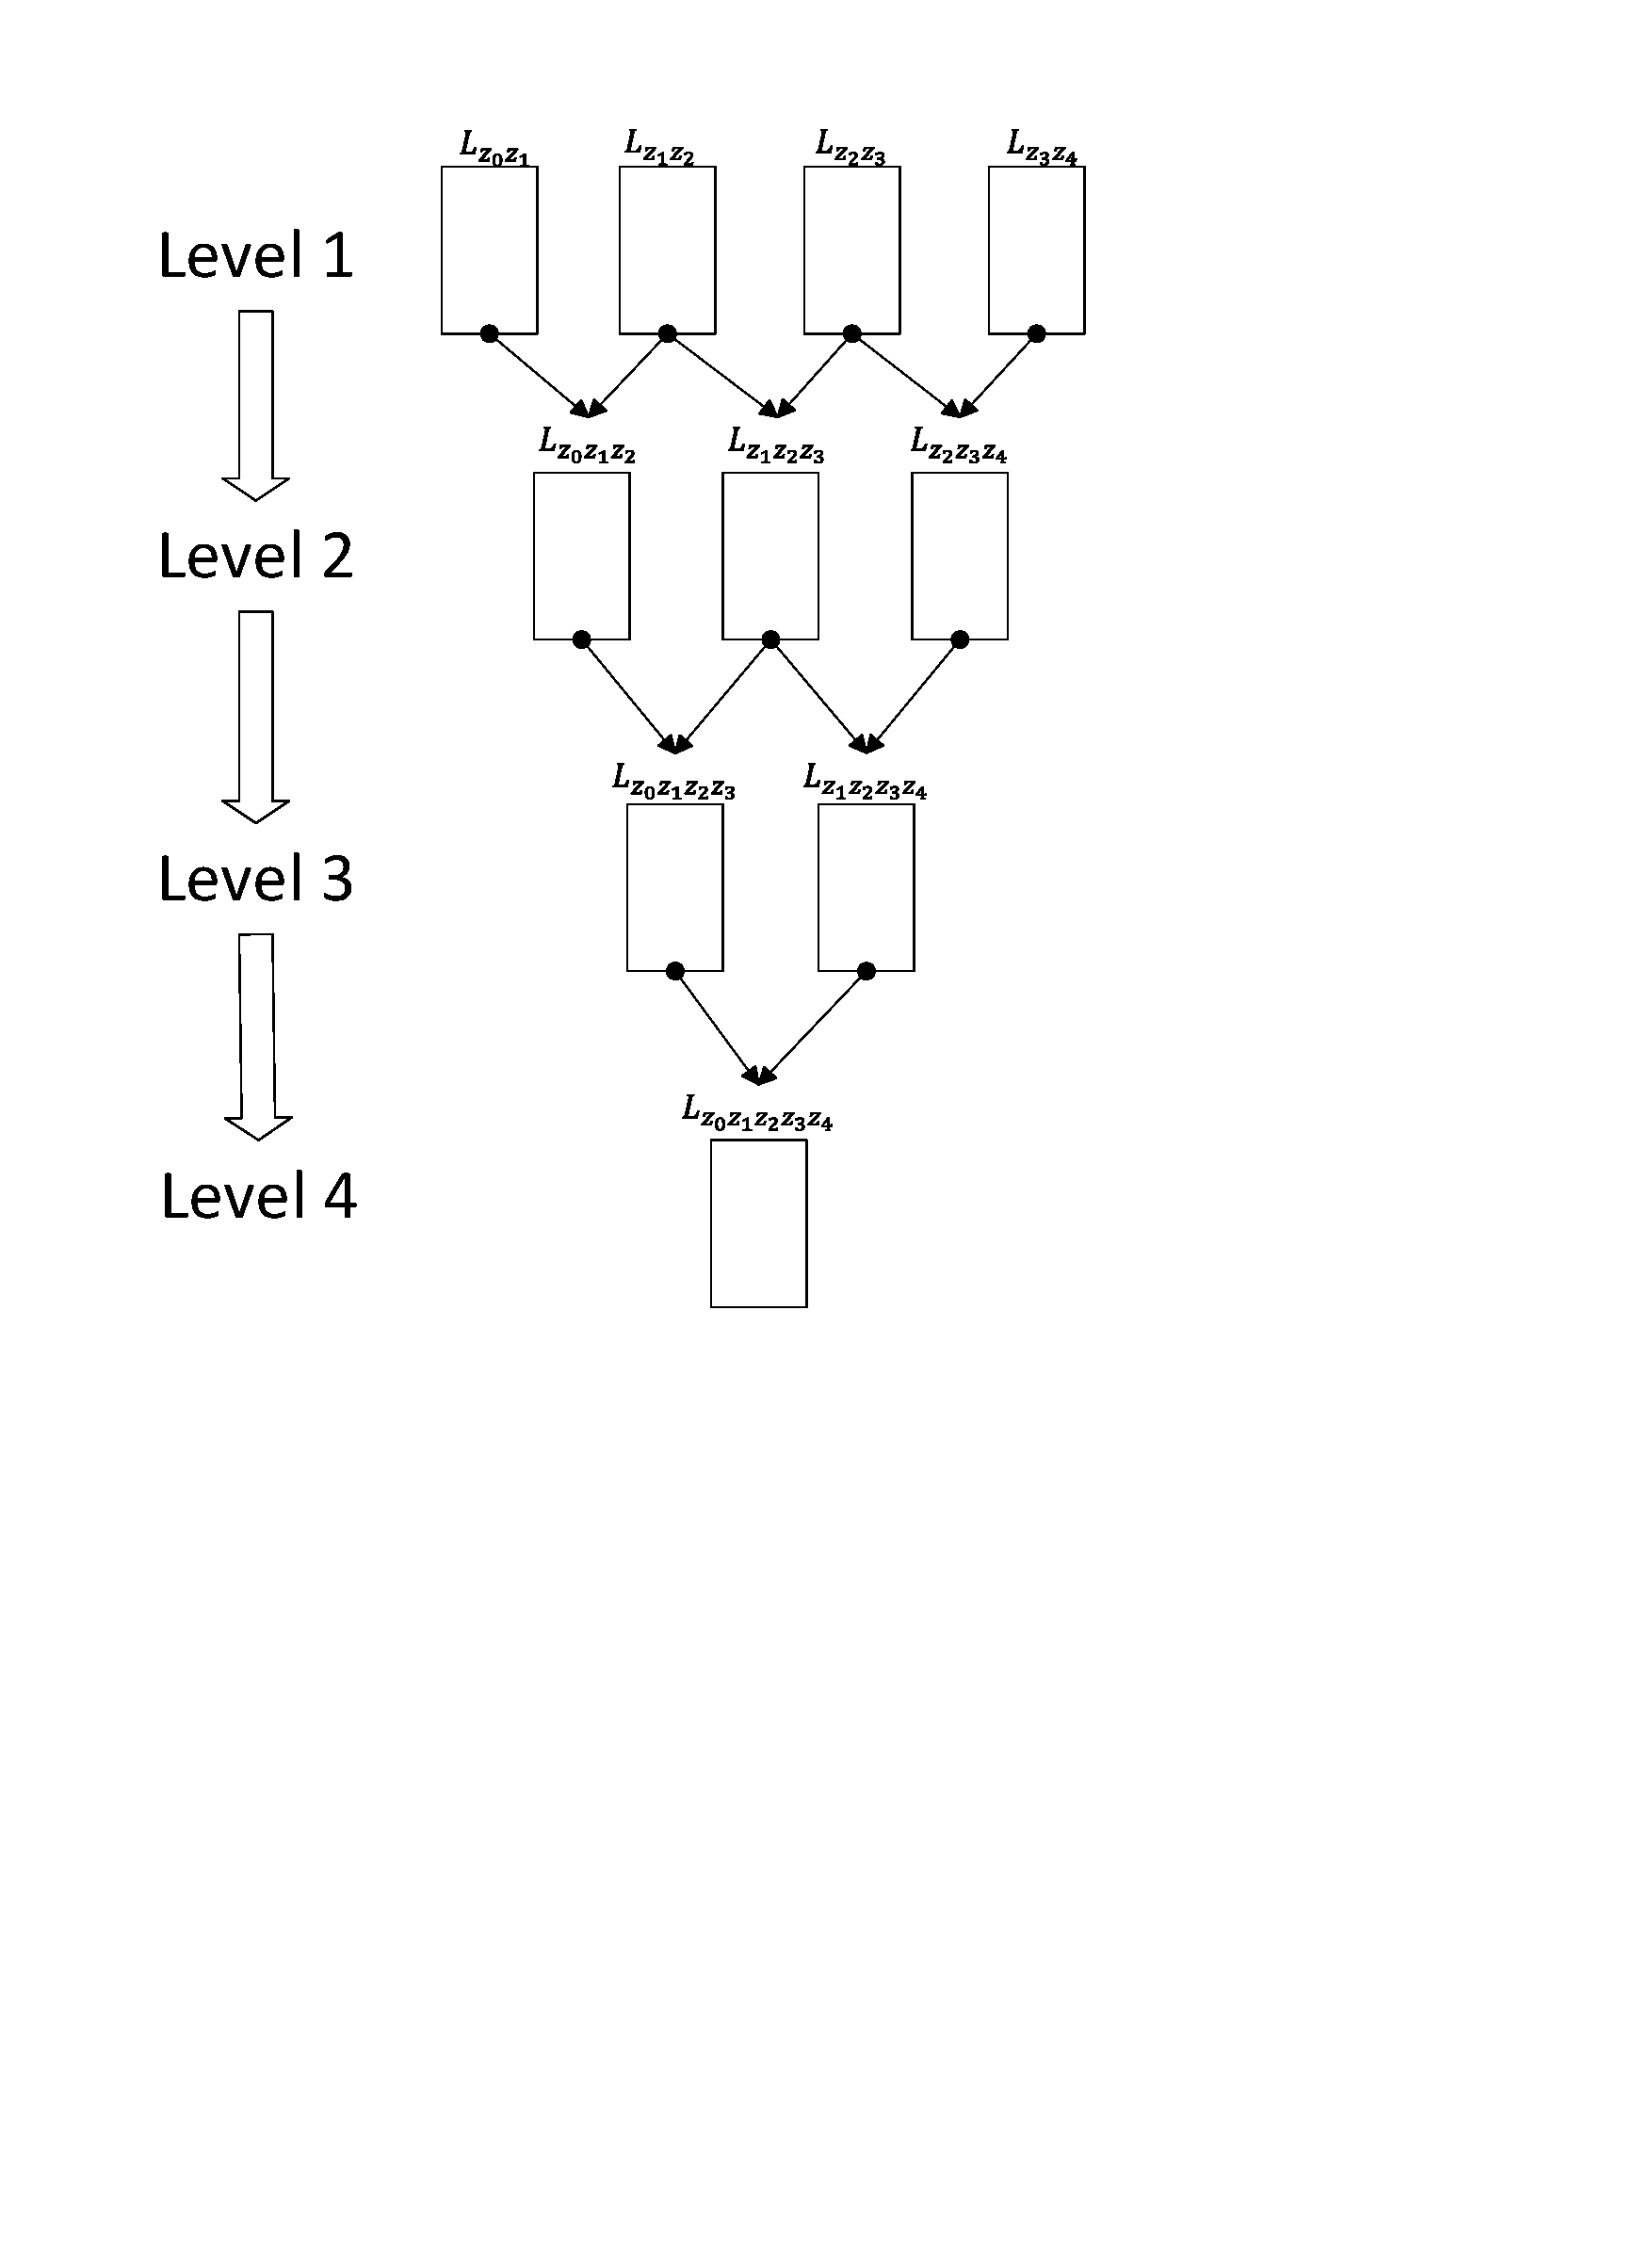
\includegraphics[width=0.5\textwidth]{pic/MergeZhang.pdf}
  \caption{The general process of Zhang's attack in \cite{AC:Zhang19}}\label{fig:MergeZhang}
\end{figure}
The 4 lists $L_{z_0z_1},\ldots, L_{z_3z_4}$ are generated by Alg.5 and are of sizes 7835 according to \cite{AC:Zhang19} (such sizes are to be corrected to 7948 according to our experiments in Table \ref{tab:ProbInU}).
Zhang has not fully implement their attack.
\cite{AC:Zhang19} only implement the steps from Level 1 to 2.
They simply gives three claims as follows:
\begin{description}
  \item[Claim 1] The whole merging process in Fig. \ref{fig:MergeZhang} requires $2^{28.3}$ cipher ticks.
  \item[Claim 2] The final $L_{z_0z_1z_2z_3z_4}$ contains $2^{16.6}$ candidates.
  \item[Claim 3] The elements in the lists require at most 5 bytes of memory.
  \item[Claim 4] Each candidate in $L_{z_0z_1z_2z_3z_4}$ have 33 known bits.
\end{description}
Our practical implementation of the full attack proves that all the claims above are wrong.

Since the merging of two lists $L_1,L_2$ requires $|L_1|\cdot |L_2|$ operations, it is impossible to get exact evaluation to the complexities without actually knowing the sizes of all the lists.
According to our implementation, the sizes of the lists are as follows:
\begin{equation}\label{eq:ListSizes}
  \begin{aligned}
  |L_{z_iz_{i+1}}| &\approx 2^{12.95},\quad \text{ for } i=0,\ldots, 3 \\
  |L_{z_iz_{i+1}z_{i+2}}| & \approx 2^{16.70},  \quad \text{ for } i=0,\ldots, 2\\
  |L_{z_iz_{i+1}z_{i+2}z_{i+3}}| & \approx 2^{20.46},  \quad \text{ for } i=0,\ldots, 1\\
  |L_{z_0z_{1}z_{2}z_{3}z_{4}}| & \approx 2^{24.21}
  \end{aligned}
\end{equation}
Therefore, the complexity of the merging process is dominated by Level 3 to 4 which is approximately $2^{20.46\cdot 2}=2^{40.92}$: far beyond $2^{28.3}$.
Zhang \etal's Claim 1 is wrong.
The size of $L_{z_0z_1z_2z_3z_4}$ is $2^{24.21}> 2^{16.6}$.
So Zhang \etal's Claim 2 is also wrong.
The merging process in Fig. \ref{fig:MergeZhang} takes two lists denoted as $L_t$ and $L_{t+1}$ where $L_{t}$ contains the partial states of $\vec{ s^t}$ while $L_{t+1}$ consists of partial states of $\vec{s^{t+1}}$.
According to Section \ref{sec:MovePatternAndBC}, a $\vec{s^t}$ should take a move $m_t\in \{0,1,2,3\}$ before reaching $\vec{s^{t+1}}$ and that move $m_t$ is decided by the three bits $(\vec{s^t}[8],\vec{s^t}[29],\vec{s^t}[51])$.
So the merging phase between $L_t$ and $L_{t+1}$ are as follows:
\begin{enumerate}
  \item Initialize the merged list $L_{t}'\leftarrow \phi$.
  \item For each $(\vec{s^t},\vec{s^{t+1}})\in L_t\times L_{t+1}$, do the following steps:
  \begin{enumerate}
    \item Identify the positions of the known bits in $\vec{s^t}$ denoted as $\lambda_0\subseteq [0,63]$.
    \item Determine the move $m_t$ according to 3 known bits of $\vec{s^t}$ namely $(\vec{s^t}[8],\vec{s^t}[29],\vec{s^t}[51])$.
    \item Determine the state $\vec{\hat{s}^t}$ \st $\vec{\hat{s}^t}\xrightarrow[]{m_t} \vec{s^{t+1}}$.
    \item Identify the positions of the known bits in $\vec{\hat{s}^t}$ denoted as $\lambda_1\subseteq [0,63]$.
    \item If $\vec{\hat{s}^t}[\lambda_0\cap \lambda_1]=\vec{s^t}[\lambda_0\cap \lambda_1]$, store the vector $\vec{\tilde{s}^t}\leftarrow \vec{\hat{s}^t} \vee \vec{s^t}$ where $\vee$ is bitwise OR.
        The known bits of the newly generated  $\vec{\tilde{s}^t}$ is $\tilde{\lambda}\leftarrow\lambda_0\cup \lambda_1$.
  \end{enumerate}
\end{enumerate}
According to the description above, any element $\vec{s}\in L$ should not only contain the value but the  positions of the known bits as well.
At Level 1, since all list are generated through Alg3, all elements share the same known-bit positions
\begin{equation}\label{eq:KnownBitsL1}
\lambda=\{7,8,16,17,18,  28,29,38,39,40,  50,51,61,62,63\}
\end{equation}
But the following Example \ref{examp:DifferentMoveKnownBits} shows that different moves will result in different known bit positions. 
Example \ref{examp:DifferentMoveKnownBits} indicates that the known bits of the merged partial state $\vec{\tilde{s}^t}$ may not be exactly the 21 bits given in \cite{AC:Zhang19}: they are also likely to be subsets of the 21 bits.
\begin{example}\label{examp:DifferentMoveKnownBits}
  Let $(\vec{s^0},\vec{s^1})\in L_{z_0z_1}\times L_{z_1z_2}$.
  We have $\lambda_0=\lambda$ in \eqref{eq:KnownBitsL1}.
  If the move is $m_0=0$ ($(\vec{s^0}[8], \vec{s^0}[29], \vec{s^0}[51])\in \{(0,0,0),(1,1,1)\}$), we have
  \[
  \lambda_1:=\{7-1,8-1,16-1,17-1,18-1,   28-1,29-1,38-1,39-1,40-1,  50-1,51-1,61-1,62-1,63-1  \}.
  \]
  and $|\tilde{\lambda}|=21$. 
  If the move is $m_0=1$, ($(\vec{s^0}[8], \vec{s^0}[29], \vec{s^0}[51])\in \{(1,0,0),(0,1,1)\}$), we have
  \[
  \lambda_1:=\{7,8,16,17,18,   28-1,29-1,38-1,39-1,40-1,  50-1,51-1,61-1,62-1,63-1  \}.
  \]
    and $|\tilde{\lambda}|=19$.
\end{example}
In order to keep merging the lists in Level 2-4, $\tilde{\lambda}$ containing the known bit positions should also be stored taking the same size of the partial states.
Since the lists in Level 4 contain partial states of 33 bits, the $\tilde{\lambda}$'s are of the same size of 33 bits.
So the elements in the lists requires at most $\lceil 2\cdot 33/8\rceil=9$ bytes: Zhang \etal's Claim 3 is wrong.
Same with Example \ref{examp:DifferentMoveKnownBits}, the $\tilde{\lambda}$ for $\vec{\tilde{s^t}}\in L_{z_0z_1z_2z_3z_4}$ are more likely to be subsets of the 33 bits: Claim 4 of Zhang \etal is wrong.
In fact, according to our experiments, the number of known bits of $L_{z_0z_1z_2z_3z_4}$ elements are usually $|\tilde{\lambda}|\approx 30$, which is far below 33.

\subsection{The Corrected Complexities of Zhang \etal's Attack}
According to Zhang \etal in \cite{AC:Zhang19}, after the CP part in $L_{z_0z_1z_2z_3z_4}$ are recovered, the rest parts are to be recovered in the same manner as our guess-and-determine attack in Section \ref{sec:OurGuessAndDetermine}: for each $\vec{\tilde{s}^0}\in L_{z_0z_1z_2z_3z_4}$, we deduce the moves $m_0,\ldots, m_4$, guess moves $m_t$ for $t=5,6,7,...$ and maintain a bit condition system in \eqref{eq:BCLpSystem} to identify the correct state.
It is also noticeable that the system $A\vec{x}^T=b^T$ should not only contain the $3t$ bit conditions deduced from $(m_0,\ldots, m_t)$ and $(z_0,\ldots, z_t)$: there are also $|\tilde{\lambda}|$ bit conditions identifying the known bits for $\vec{\tilde{s}^0}\in L_{z_0z_1z_2z_3z_4}$. 
So the number of bit conditions should now become $3t+|\tilde{\lambda}|$. 
So the whole process of Zhang \etal's attack can now be summarized as follows:
\begin{enumerate}
  \item Query the A5/1 encryption oracle for $\ell$ keystream bits $z^0,\ldots, z^{\ell}$
  \item Run the merging process in Fig. \ref{fig:MergeZhang} and acquire the list of candidates $L_{z_0z_1z_2z_3z_4}$ for the CP part of A5/1.
   \item Initialize an empty set $\mathcal{S}$ of $\vec{s^0}$ candidates
   \item For each $\vec{\tilde{s}^0}\in L_{z_0z_1z_2z_3z_4}$
   \begin{enumerate}
     \item Deduce the 5 moves $(m_0,\ldots, m_4)$ and the known bit position set $\tilde{\lambda}$
     \item For some $t \in [6,\ell)$, we guess the $2^{2(t-5)}$ movements $(m^5,\ldots, m^t)$, we acquire the bit conditions $\mathcal{BC}\leftarrow {\tt getBC}((m^0,\ldots, m^t), (z^0,\ldots, z^t))$ and do the following substeps:
     \begin{enumerate}
        \item For all $i\in \tilde{\lambda}$, add the bit condition $x_i=\vec{\tilde{s}^0}[i]$ to $\mathcal{BC}$
        \item Deduce the $A$ and $\vec b$ in \eqref{eq:BCLpSystem} according to $\mathcal{BC}$ and compute the extended matrix $E$ in \eqref{eq:ExtendedMatrixOfA}
        \item Compute $order(A)$ and $order(E)$, if $order(A)\neq order(E)$, such a movement guess is wrong, go back to Step 2 for the next movement guess
        \item For all $2^{64-order(A)}$ solutions to $A\vec x^T=b^T$, set $\vec{\hat{s}^0}\leftarrow \vec x$ and generate the keystream bits $\hat{z}^0,\ldots, \hat{z}^t,\hat{z}^{t+1},\ldots, \hat{z}^{\ell}$
        \item If $(\hat{z}^{t+1},\ldots, \hat{z}^{\ell})=(z^{t+1},\ldots, z^{\ell})$, add such $\vec{\hat{s}^0}$ into $\mathcal{S}$
      \end{enumerate}
   \end{enumerate}
  \item Return $\mathcal{S}$
\end{enumerate}

\noindent\textbf{Complexity Analysis. }
In Step 4.(b), there are $2^{2t-10}$ candidate moves $(m^0,\ldots, m^{t})$ and we assume that only $\alpha 2^{2t-10}$ moves can pass the $order(A)=order(E)$ test at Step 4.(b).iii where $0\leq \alpha \leq 1$.
We denote the averaging $order(A)$ as $\beta $.
According to \eqref{eq:ListSizes}, the size of $L_{z_0z_1z_2z_3z_4}$ is approximately $2^{24.21}$. 
The analysis in Section \ref{sec:ZhangWrongCompAnalysis}, the merging process in Step 2 has complexity $2^{40.92}$.
With $\alpha ,\beta $, the averaging time complexity can be computed as \eqref{eq:ZhangComplexityCorrect}. 
\begin{equation}\label{eq:ZhangComplexityCorrect}
\begin{aligned}
Comp&=2^{40.92}+2^{24.21+2t-10}+\alpha \cdot 2^{24.21+2t-10+64-\beta}\\
&=2^{40.92}+2^{14.21+2t}+2^{78.21+\log \alpha -\beta}
\end{aligned}
\end{equation}
Same with Section \ref{sec:MovePatternAndBC}, we randomly select $2^{30}$ $\left(\vec{\tilde{s}^0}, (m^5,\ldots, m^t), (z^5,\ldots, z^m)\right)$ triplets and do the 4.(b).iii test to compute the averaging $\alpha$ and $\beta$ for $t$'s.
For $6\leq t\leq 29$, the $\alpha$, $\beta$ and $Comp$ are listed in Table \ref{tab:ZhangAlphaAndBeta}.
As can be seen, the lowest complexity appears at $t=xxxxxx$ with $Comp=2^{xxxxx}$. 
The memory complexity is dominated by the size of $L_{z_0z_1z_2z_3z_4}$ which is $2^{24.21}$ according to \eqref{eq:ListSizes}. 
Zhang \etal has already claimed that the attack can only succeed when the exact $\vec{s^i}$ lies in the corresponding list $L_{z_iz_{i+1}}$ for $i=0,1,2,3$ in Fig. \ref{fig:MergeZhang}. 
According to the Section \ref{sec:ZhangWrongP1}, the success probability can be evaluated as $p_1^4\approx 0.8942$. 


\begin{table}[htbp]
  \centering
  \caption{The averaging $\alpha$ and $\beta$ in \eqref{eq:Complexity} with $2^{30}$ random tests}\label{tab:ZhangAlphaAndBeta}
    \begin{tabular}{|l|l|l|l|l|l|l|l|}
    \hline
    \multicolumn{1}{|c|}{$t$} & \multicolumn{1}{c|}{$\beta$} & \multicolumn{1}{c|}{$\log\alpha$} & \multicolumn{1}{c|}{$\log Comp$} & \multicolumn{1}{c|}{$t$} & \multicolumn{1}{c|}{$\beta$} & \multicolumn{1}{c|}{$\log\alpha$} & \multicolumn{1}{c|}{$\log Comp$} \\
    \hline

    5    & 41.95852 & -0.02809 & 50.01338 & 22    & 61.60404 & -3.97115 & 44.41749 \\
    \hline
    6    & 44.86764 & -0.09501 & 49.03736 & 23    & 62.78097 & -5.91544 & 46.0546 \\
    \hline
    7    & 47.68339 & -0.23144 & 48.08519 & 24    & 63.43321 & -8.4195 & 48.00623 \\
    \hline
    8    & 50.38127 & -0.46833 & 47.15056 & 25    & 63.75542 & -11.173 & 50.00074 \\
    \hline
    9    & 52.95498 & -0.81293 & 46.23329 & 26    & 63.9043 & -14.0599 & 52.00009 \\
    \hline
    10    & 55.4087 & -1.26981 & 45.33048 & 27    & 63.96694 & -17.0267 & 54.00001 \\
    \hline
    20    & 57.73363 & -1.85176 & 44.48072 & 28    & 63.98999 & -20.0213 & 56 \\
    \hline
    21    & 59.86026 & -2.67122 & \textbf{43.91356} & 29    & 63.99728 & -23.1174 & 58 \\
    \hline

    \end{tabular}%
\end{table}%





\section{Conclusion}





\ifLNCSVER
  \bibliographystyle{splncs}
\else
  \bibliographystyle{alpha}
\fi
\bibliography{bib/abbrev3,bib/crypto,myrefs}




\ifLNCSVER

\else

\fi



\end{document}

